\documentclass[tikz,border=8pt]{standalone}
\usepackage{amsmath}
\usetikzlibrary{arrows.meta,positioning,calc}

\begin{document}
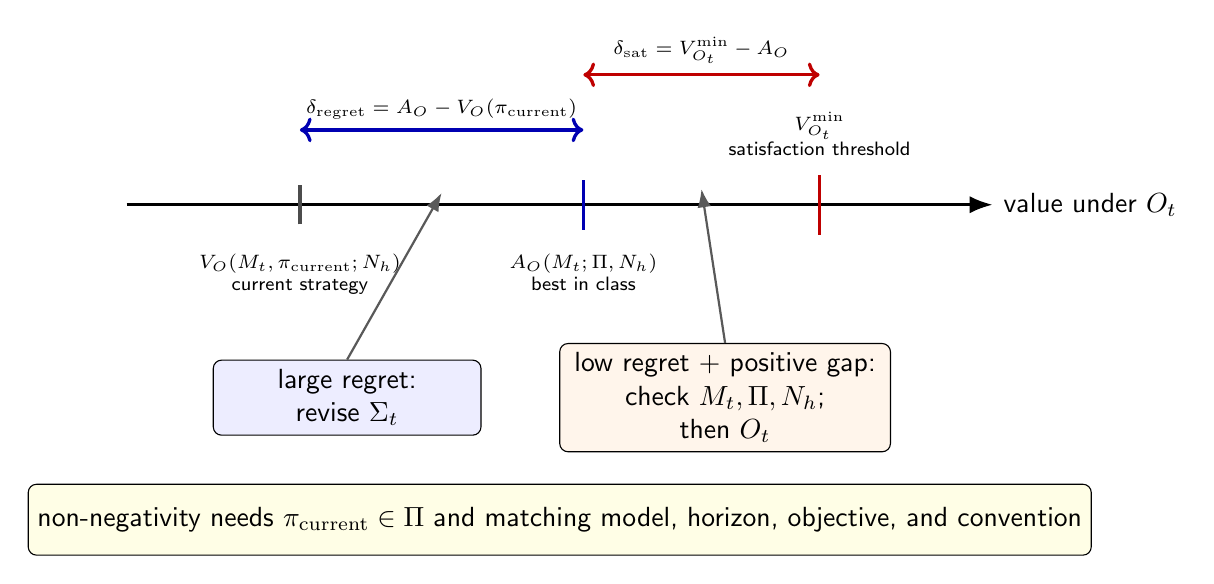
\begin{tikzpicture}[
  font=\sffamily,
  note/.style={align=center, font=\sffamily\scriptsize},
  labelbox/.style={draw, rounded corners=3pt, align=center, fill=white, minimum height=9mm},
  arrow/.style={-Latex, thick, draw=black!65},
  interval/.style={<->, very thick}
]

\draw[-Latex, very thick] (0,0) -- (11,0) node[right] {value under $O_t$};

\coordinate (cur) at (2.2,0);
\coordinate (best) at (5.8,0);
\coordinate (thr) at (8.8,0);

\draw[very thick, draw=black!70] (cur) ++(0,-0.25) -- ++(0,0.5);
\draw[very thick, draw=blue!70!black] (best) ++(0,-0.32) -- ++(0,0.64);
\draw[very thick, draw=red!75!black] (thr) ++(0,-0.38) -- ++(0,0.76);

\node[note, below=5mm] at (cur) {$V_O(M_t,\pi_{\rm current};N_h)$\\current strategy};
\node[note, below=5mm] at (best) {$A_O(M_t;\Pi,N_h)$\\best in class};
\node[note, above=5mm] at (thr) {$V_{O_t}^{\min}$\\satisfaction threshold};

\draw[interval, draw=blue!70!black] ($(cur)+(0,0.95)$) -- node[above, note] {$\delta_{\rm regret}=A_O - V_O(\pi_{\rm current})$} ($(best)+(0,0.95)$);
\draw[interval, draw=red!75!black] ($(best)+(0,1.65)$) -- node[above, note] {$\delta_{\rm sat}=V_{O_t}^{\min}-A_O$} ($(thr)+(0,1.65)$);

\node[labelbox, fill=blue!7, minimum width=34mm] (strategy) at (2.8,-2.45)
  {large regret:\\revise $\Sigma_t$};
\node[labelbox, fill=orange!8, minimum width=42mm] (capability) at (7.6,-2.45)
  {low regret + positive gap:\\check $M_t,\Pi,N_h$;\\then $O_t$};

\draw[arrow] (strategy.north) -- ($(cur)!0.5!(best)+(0,0.15)$);
\draw[arrow] (capability.north) -- ($(best)!0.5!(thr)+(0,0.2)$);

\node[labelbox, fill=yellow!10, minimum width=92mm] at (5.5,-4.0)
  {non-negativity needs $\pi_{\rm current}\in\Pi$ and matching model, horizon, objective, and convention};

\end{tikzpicture}
\end{document}
